\documentclass[12pt]{article}
\usepackage[margin=1in]{geometry}
\usepackage{amsmath}
\usepackage{graphicx} % for \includegraphics (see the note below)
\usepackage{tikz}     % lets us draw a figure with no external image file

\title{Figures and Cross-References}
\author{Your Name}
\date{\today}

\begin{document}
\maketitle

\section{Referring to things by number}

Give anything numbered a \verb|\label|, then point at it with
\verb|\ref| (or \verb|\eqref| for equations). LaTeX fills in the number
and keeps it correct when things move.

Equation~\eqref{eq:euler} relates five constants:
\begin{equation} \label{eq:euler}
    e^{i\pi} + 1 = 0.
\end{equation}

\section{Figures}

A \texttt{figure} floats to a convenient spot and its \verb|\caption| is
numbered. The figure below is drawn with TikZ, so no image file is
needed. To drop in an image file instead, replace the
\texttt{tikzpicture} with, for example,
\verb|\includegraphics[width=0.4\textwidth]{myplot.png}|.

\begin{figure}[ht]
    \centering
    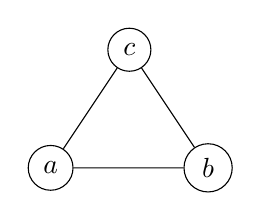
\begin{tikzpicture}
        \node[circle, draw] (a) at (0, 0)   {$a$};
        \node[circle, draw] (b) at (2, 0)   {$b$};
        \node[circle, draw] (c) at (1, 1.5) {$c$};
        \draw (a) -- (b) -- (c) -- (a);
    \end{tikzpicture}
    \caption{A triangle on three vertices.}
    \label{fig:triangle}
\end{figure}

Figure~\ref{fig:triangle} shows the graph. You never type the numbers
yourself --- add a figure earlier in the document and every later
reference renumbers on the next compile. The \verb|~| in
\verb|Figure~\ref{...}| is a non-breaking space, so the word and its
number never split across a line.

\end{document}
